Robotics has always been an appealing research field for many
application fields. Since the first industrial revolution, machinery
has been built in order to automate repetitive tasks which had been
completed by humans before that moment. This process brought the
entire humanity to change its way of life, bringing the main part of
society from an agricultural, artisanal system to a modern,
industrialized one. In general, this has been pointed out as one of
the biggest turns in the human history, which changed almost every
aspect of people's life; although many changes due to the automation
processes have been seen as catastrophic by some, such as
\cite{bombarolo} and \cite{extinction}, mainly because of the
increased gap between wealthy countries and poorest ones, it is
undeniable that the increase of material richness which has come as a natural
consequence of all of this is a great benefit for any person.

In the first century since industrial revolution, research on
automation has focused on applying new technological discoveries to
special-purpose machines; this has brought to automating tasks like
cloth washing, objects' manufacturing, and warehouses' management.

However, this approach has shown its drawbacks in recent times: having
a different machine for each single task, especially in case of
factory automation ones, pays a lot in terms of flexibility of the
machine itself, and this brings a much higher cost in the scenario,
which is going to be actually very common in the near future, in which
a factory wants to automate its whole structure. Also, recent
technological improvements have lowered a lot the need of
mechanics-based machinery, preferring solutions based on electronics
and complex software. This allowed a further push on automatic tasks'
completion by reducing a lot the cost of machinery (expect for
non-recurring engineering costs) due to limited material cost, which
are the most important to optimize in a world based on
mass-production. Thus, research on automation has moved to find a
solution for completing general tasks, in order to obtain, in the far
future, a robotic product which will have the ability to substitute
almost completely humans in labour.

The main research projects operating with this goal have, for obvious
reasons, focused their efforts on the study of \emph{humanoid
  robotics}, as the human body is, by an engineering point of view,
one of the most optimized, general-purpose machines in existence,
being capable of directly fulfilling extremely complex tasks, except for the
ones needing extreme precision or strength to complete. From this point of view, a
robot able to compare with the human brain in terms of decision capabilities
would make the general automation task totally completed, bringing to
the complexity of human intelligence the added value of virtually
infinite working strength and precision, due to its ad-hoc mechanical
and electronic components.

One of the main application fields in which human-like robotic devices
have always had their space is the one of objects' manipulation. In
fact, since the beginning many automatisation tasks involving
nontrivial handling of items, notably pick-and-place into
manufacturing pipelines, have been solved by usage of human-like
robotic arms, which for this reason gained their own industrial sector
since the early '70s, with the birth of companies like the Italian COMAU,
producing industrial automation solutions from the start, and the
expansion of others like the German KUKA, which moved its commercial
focus from the production of goods for manual use (wielding equipment,
communal vehicles) to the development of automated industrial robots,
which lead to the production of the first 6-DOF electric robot, named
\emph{FAMULUS}, in 1973.\footnote{http://www.kuka-robotics.com/usa/en/company/group/milestones/1973.htm}

Picking objects has thus always been a fundamental task for all of this
scenarios, and can nowadays be considered fully solved in most
cases. However, this are again all special-purpose solutions: most of
these solution are built for situations in which the pose of the
objects which will have to be manipulated is known a priori, as they
are often coming from a preceding section of a production pipeline,
and the set of movement which the object will have to do is fixed
too. Thus, an ad-hoc solution can be studied and built, and the robot
can be thought, built and programmed to fulfil robustly its unique
task. The more general manipulation scenario, in which a robot is able
to be instructed at runtime to which object to take, how to manipulate
it, and where to find it, is far beyond the current state of the art
in robotics. Nevertheless, research is growing more and more
quickly on this topic; it would, in fact, lead to virtually infinite
new opportunities for a lot of fields. One of the most important use
cases for this include
the relatively recent growth of e-commerce platforms, such at the 
most known company of this sector, \emph{Amazon.com, Inc.}, or the
online retail platform \emph{Overstock.com, Inc.}, which has become
famous as the first major e-commerce platform to accept Bitcoin as a
valid currency. Automated object manipulation is, anyway, absolutely
not limited to big companies' automation systems: another utility case
is the use of mobile, robotic platforms, equipped with robotic arms,
for domotic and household tasks, either to bring further ease in
domestic work, or to help diseased people, especially if with motion
or mental impairment. In this case, a human-like robotic arm, or a
complete humanoid robot, would be for sure the best solution, as all
the domestic scenarios are naturally designed for being interacted
with humanoids.

Research on the topic of automated object picking has, by now, started
to bring interesting and promising results; for example, universal gripping systems
are being studied for robotic arms both for industrial and domestic
scenarios (which, being so different, will hardly converge to a unique
solution); for the latter, most of the systems which have been created
take their inspiration from natural gripping systems: for example, the
solution proposed by the
robotics department of the \emph{Pisa/IIT} research centre, called
\emph{SoftHAND} and introduced in \cite{pisa-softhand}, which is shown in fig.~\ref{fig:pisa-softhand}, makes
use of a single motor to close a human-like, five-fingered hand. Each
finger, just like in a human hand, is capable of small deformations in
order to get a better grip on objects. This brings goods result in
all the scenarios in which a real human hand would suitable, which in
case of domotic areas corresponds to almost everything. Human-like
grippers are, obviously, not the only solution which is in
development: other, original systems are in study, such as Empire
Robotics' \emph{Versaball}: this gripper, which is shown in
fig.~\ref{fig:versaball}, makes use of a latex sphere filled with thin
sand, combined with a pneumatic system which draws the internal air
from the sphere, thus compressing the latex: if put onto the surface of
a small, hand-pickable object, the sand will make the latex fold
perfectly the object, and when the pneumatic system is opened it will
thus close with good strength on it.

\begin{figure}[htbp]
\centering
\begin{tabular}{c|c}
  \adjustbox{valign=m}{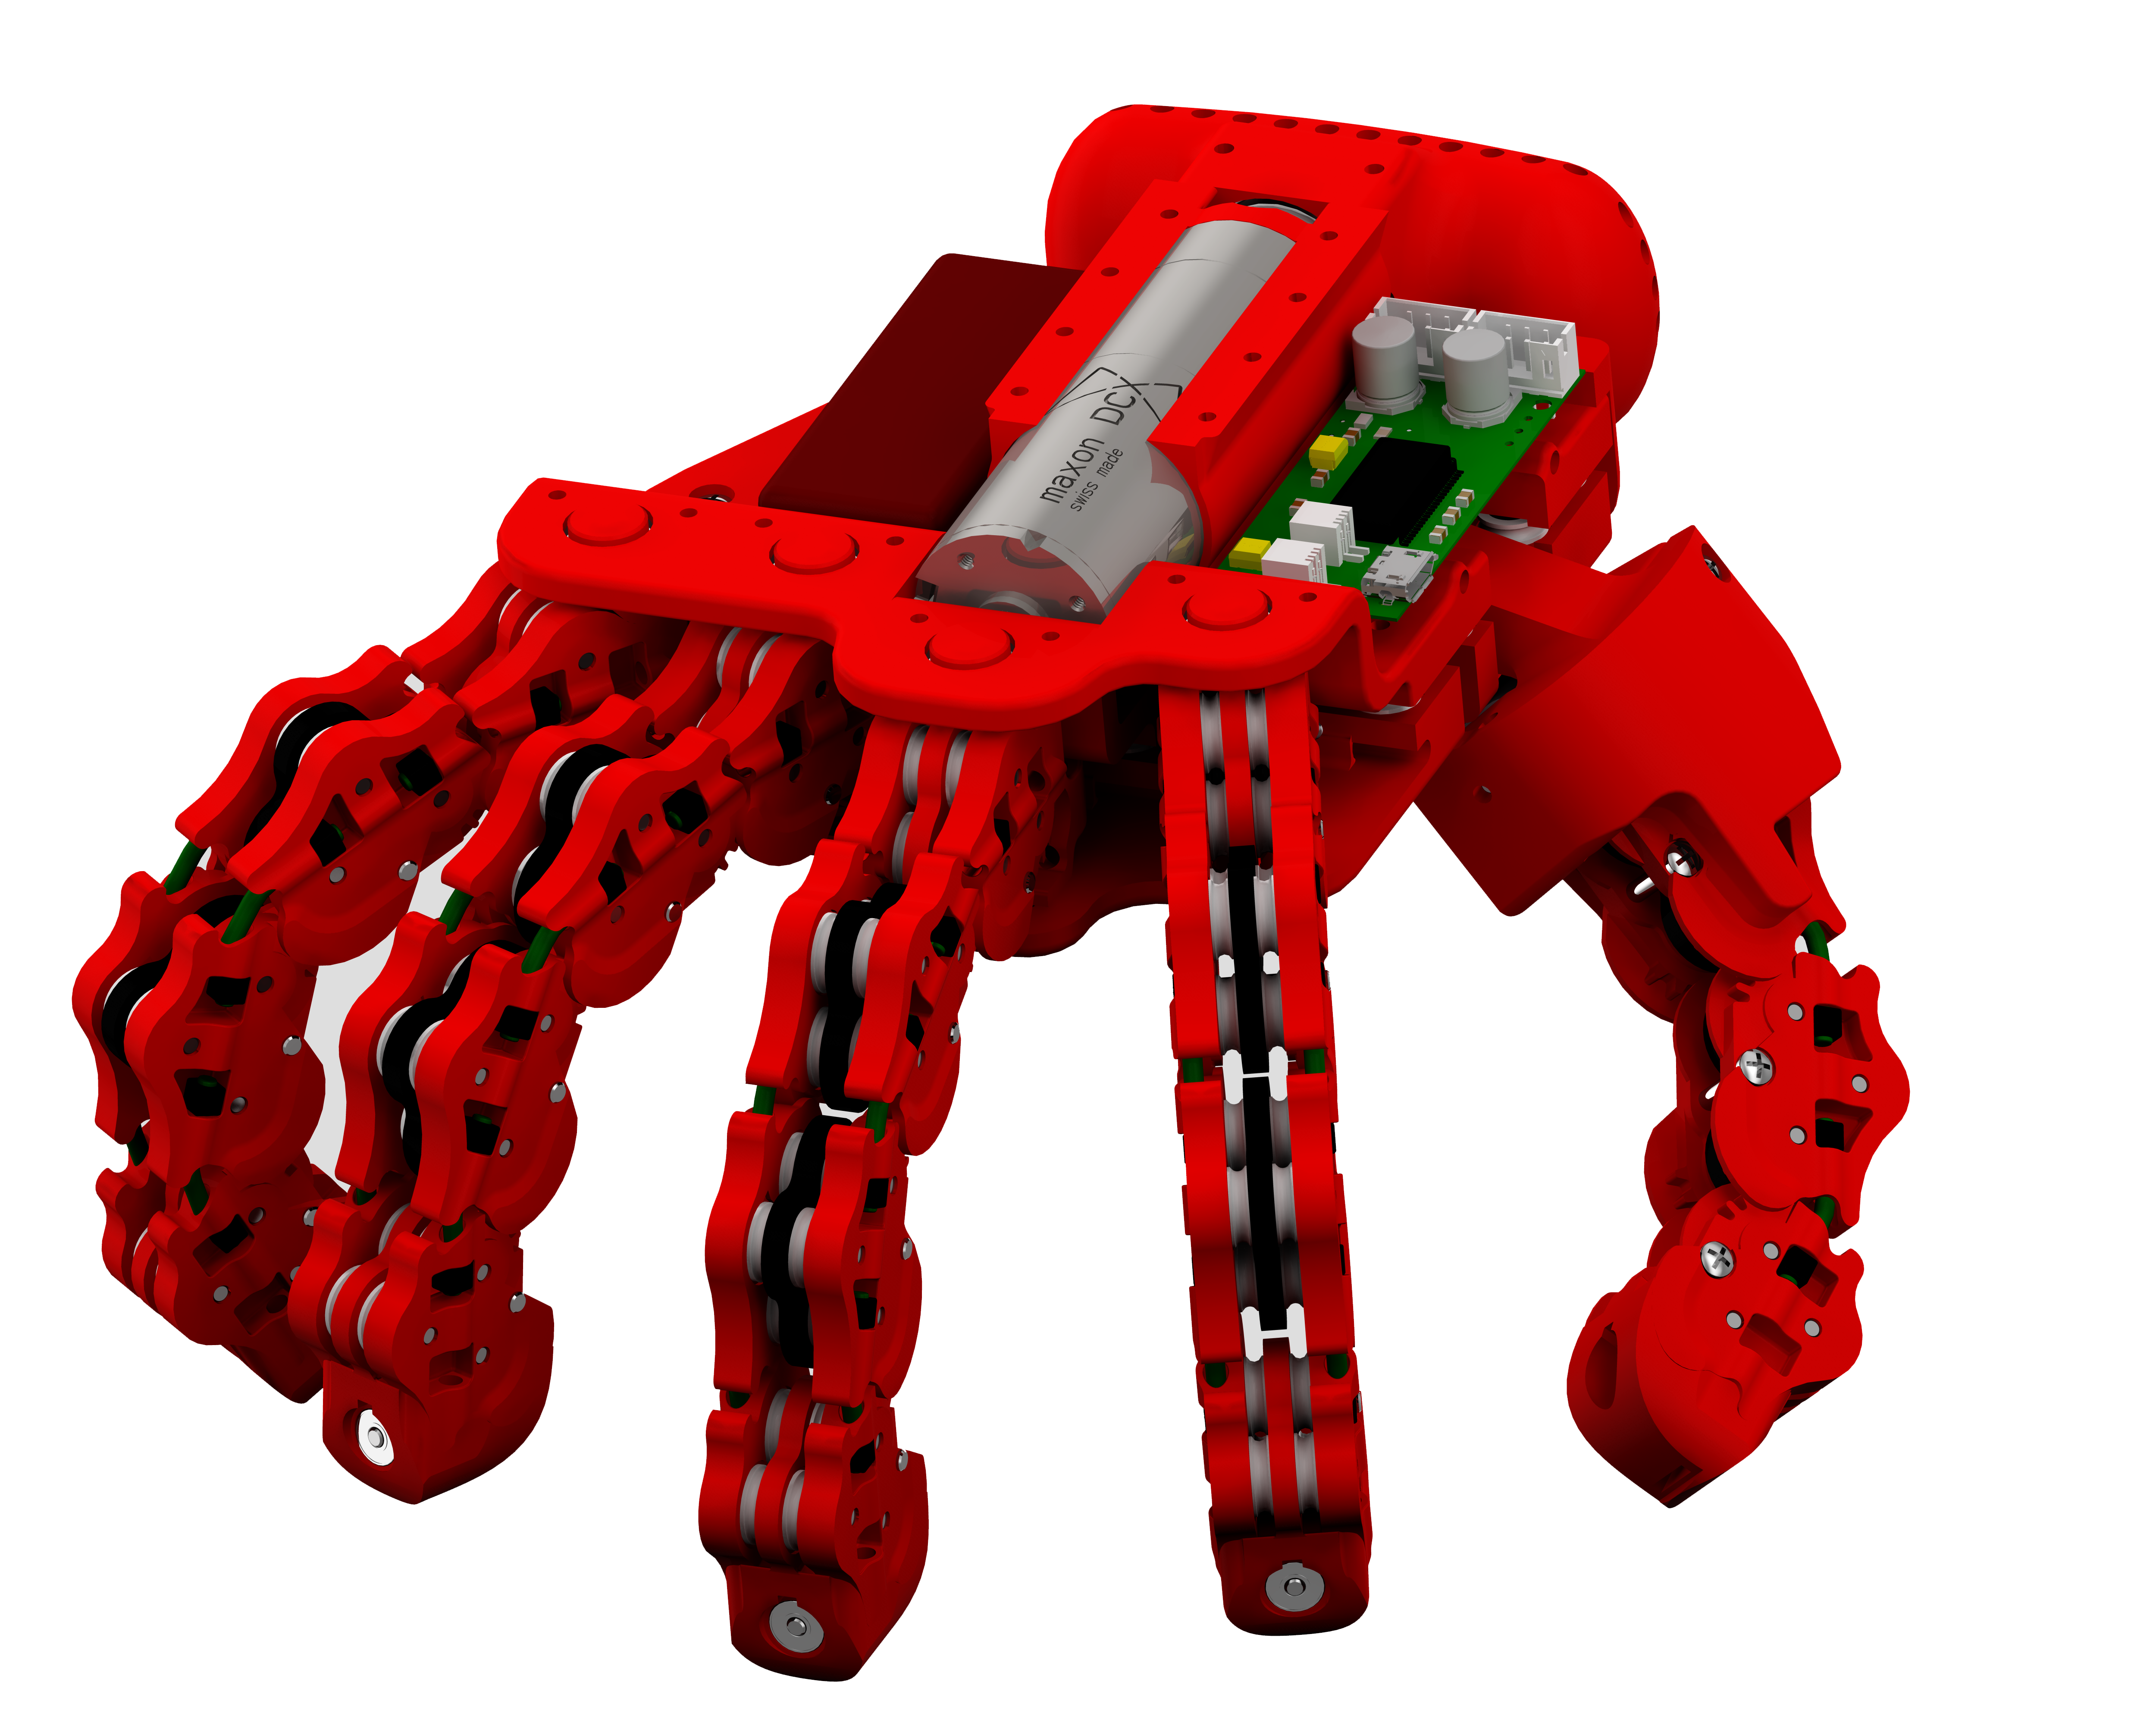
\includegraphics[width=2.5in]{./Graphics/pisa-softhand1}} &
  \adjustbox{valign=m}{\includegraphics[width=2.5in]{./Graphics/pisa-softhand2}}
\end{tabular}
\caption{Pisa/IIT's robotic gripping system, called \emph{SoftHAND},
  takes its design from the structure of a human hand, and is thus
  suitable for every task in which the latter would be. Image courtesy of Manuel Giuseppe Catalano.\label{fig:pisa-softhand}}
\end{figure}

\begin{figure}[htbp]
\centering
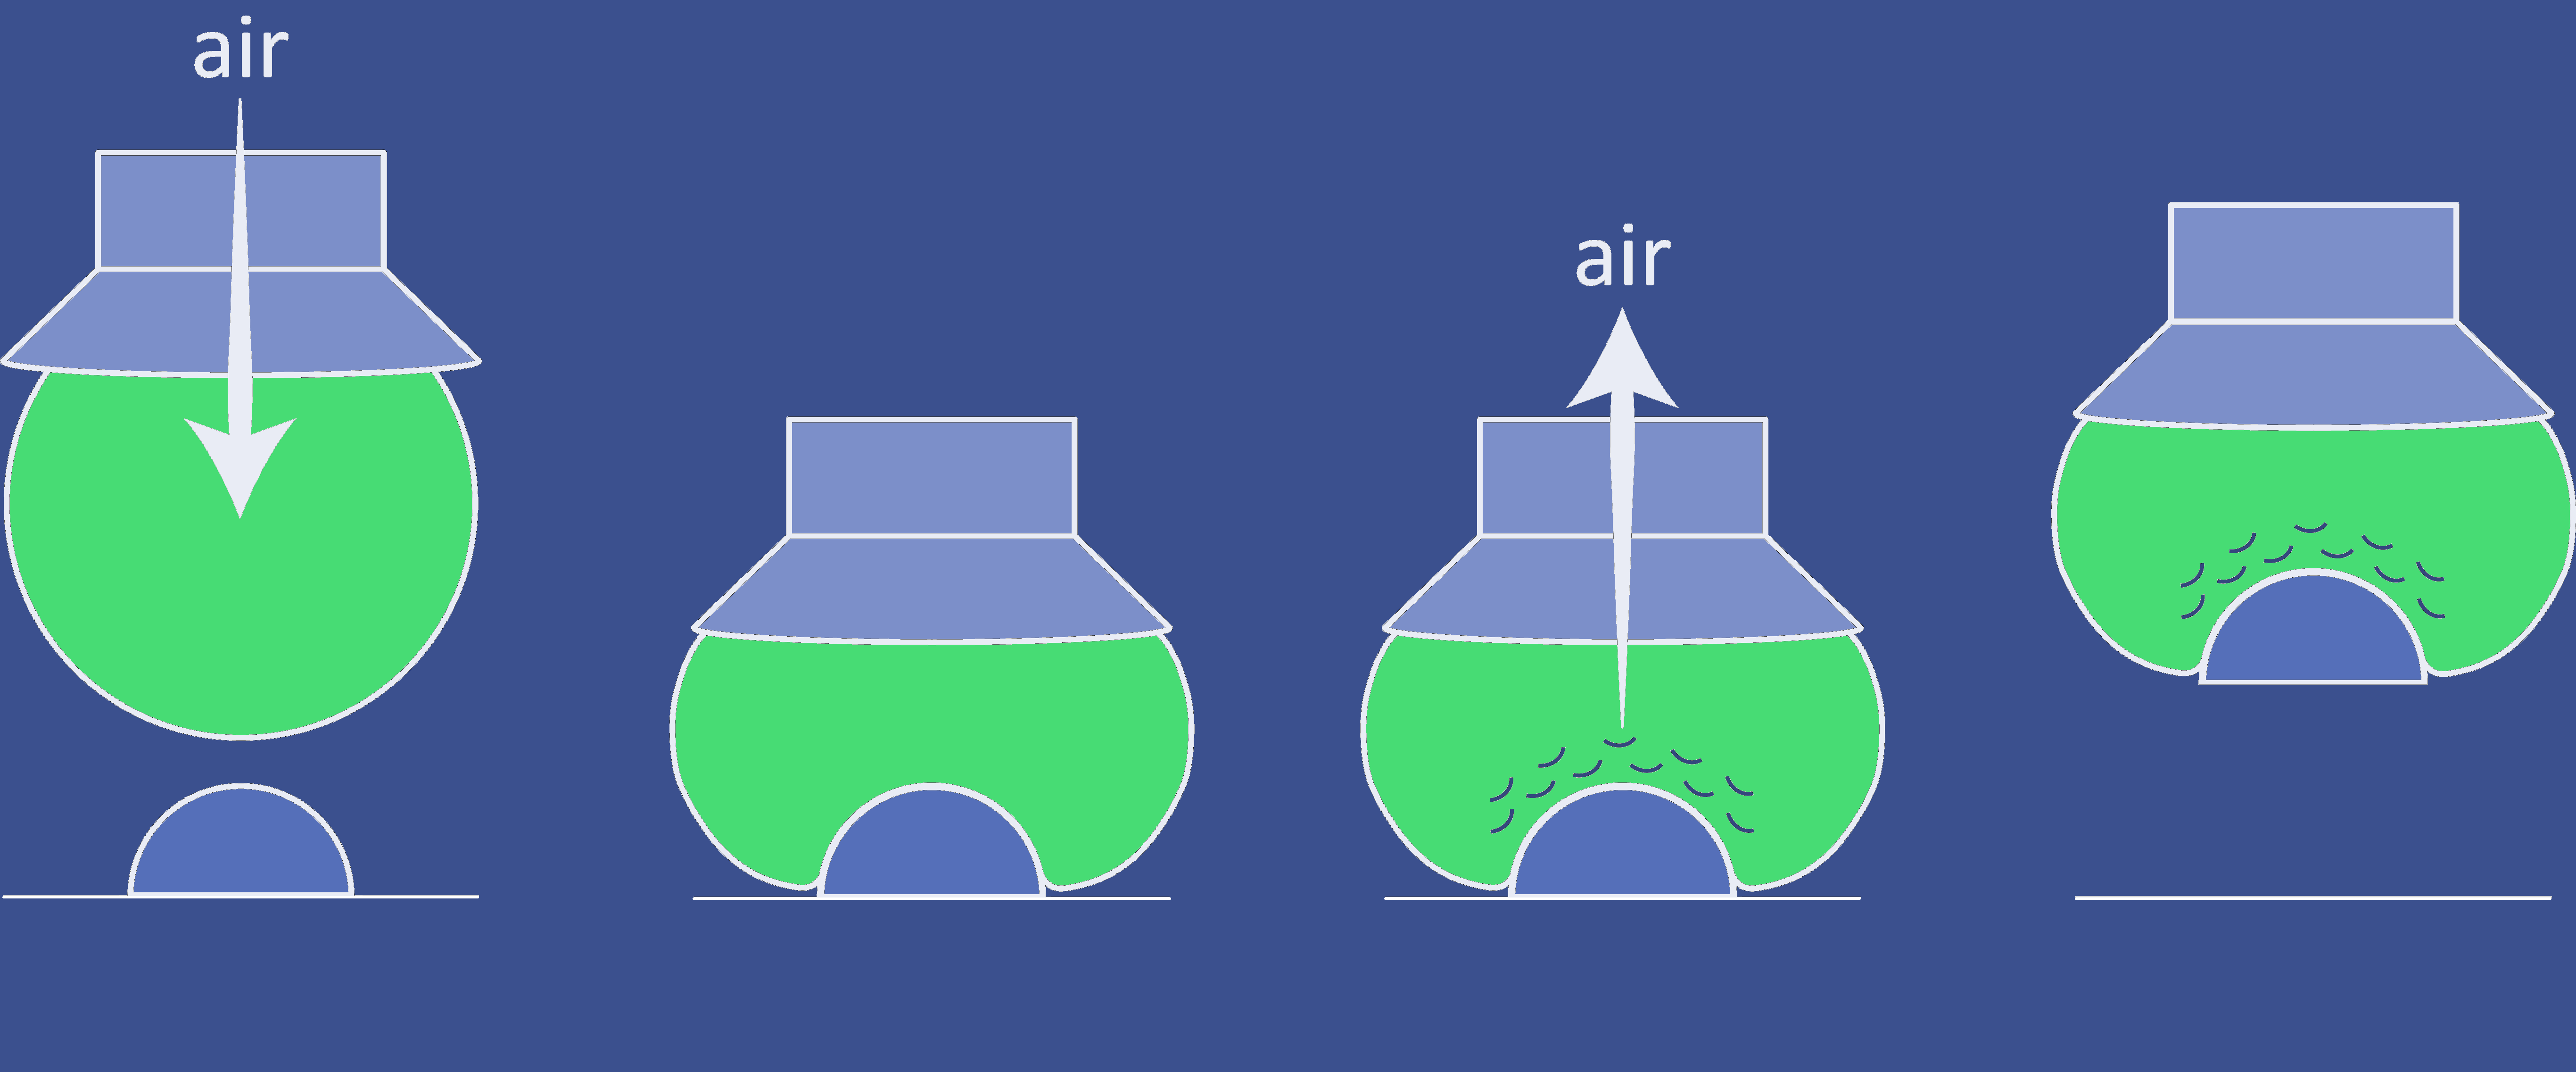
\includegraphics[width=3in]{./Graphics/versaball}
\caption{Empire Robotics' gripping system, called \emph{Versaball},
  diverges from the recent humanoid research and proposes a novel
  approach to the gripping problem. Image courtesy of Bill Culley.\label{fig:versaball}}
\end{figure}

\section{A case study for automated gripping systems: Amazon Picking
  Challenge} \label{sec:apc}
The high request of research in the field of automated objects picking
is not only a supposition, but has been proven to be a impellent need
by the financial effort that big companies are putting on this
topic. One of the most important events which has come out for this is
the \emph{Amazon Picking Challenge}, a robotics competition which saw
its first edition if June, 2015, as part of the 2015 edition of the \emph{IEEE
International Conference on Robotics and Automation (ICRA)}. This
event has brought some of the world's top-level research 
centres to show the state of the art in this field.

Being one of the biggest companies in the world, and establishing its
multi-billionaire business mainly on big volumes on electronic sales
of material goods, Amazon.com, Inc. has important and obvious interest
in selling automatization\footnote{http://www.wired.com/2014/06/inside-amazon-warehouse/}. In fact, during the last years, it has
added more and more automatic processes to their warehouses; in
particular, the whole organisational process, which receives its
material orders directly from the Amazon web selling system, is
managed totally in an automatic way, delivers its orders to the
warehouses, manages the package delivery process, and thus provides
the totality of the order fulfilment service. This huge organization,
however, still relies on a huge manpower (the Phoenix warehouses
consist of an impressive $0.1\unit{km^2}$ structure, employing more
than 1500 people); the long-term plans for it have been made evident
in recent years, being to bring full independence from human intervention for the whole
sales process: in this sense, research has first focused on investing
for the delivery path going from the destination warehouse to the
buyer's address, with the big investment made in 2013 on drones-based
systems, and the 2015 announce that perishable products would have been
made available to the final customer within one hour from order, which
started to work in the early November, 2015, in major world's
cities. As this research projects are quickly converging on a
solution, Amazon started to move on with the last -- and most
difficult -- problem which still has to be solved, which is the one of
internal automatization of warehouses, i.e. moving objects from one
place to the other into the factory and automatically package them,
using if possible the same robot which took the object from its
stocking place.

For this purpose, the contest's specifications have been made quite simple, and the plans
for future editions are to increase the difficulty level of the tasks
to be completed, in order for the best research groups to develop a
stable and robust platform which will be able to substitute the human
manpower almost completely.

The goal of this thesis project is to develop a framework for robotic
gripping like the ones proposed into this challenge; this will be able
to be extended and used as a base to build general-purpose robots
which are the aim of factory automation systems of these types.

The complete source code of this project, which complements this
thesis, together with its documentation, which comes as an integrative part to this more theoretical report, can be found at \url{github.com/Conte91/JG}.

\subsection{Amazon Picking Challenge problem statement} \label{sec:apc}
Here follows a brief description of the Amazon Picking Challenge's
specifications, which have been taken as a reference for how the robot
shall behave in a warehouse environment.

\begin{itemize}

\item{First of all, each robot is assigned a \emph{shelf} on which it will
operate; both the robot and the shelf could actually be able to move
into the warehouse (KivaPOD shelves, for example, are systems able to
move on wheels and coordinate each other in a crowded environment),
but for the purpose of focusing on the problem it will be assumed
that, when instructed to start, the robot will already be in front of
its shelf;}
\item{A shelf is made of several \emph{bins}, for which the location
into the shelf is known a priori; each bin can contain one or more
instances of objects taken from a predefined set. For this challenge,
a set of 25 items commonly sold on Amazon.com has been selected,
composed mainly by everyday items such as books, children toys, and
office equipment; each object type is uniquely identified by its ID
(multiple objects of the same type share a common ID);}
\item{Each bin is labelled with a sequential letter, starting with A,
and its content in terms of objects is known; what is not known is the
position of these objects inside their bin;}
\item{The list of items which the robot will have to grasp is defined
in a \emph{work order}, which is given as an input to the robot at
startup, as a single JSON file (app.~\ref{app:json} contains an
example of such files); for each item into the work order, both the object's ID and
the bin from which the object has to be taken are specified; it is not
possible that an item does not correspond to a real object into its
bin (i.e. bin descriptions are consistent, and no checks are needed
for this);}
\item{For each item into the work order, the robot will have to
identify the object into the correct bin, pick it, and put it into a
plastic container, representing the destination package of the
object. It is very important that the robot does not break any of the
objects into the shelf while operating, and that it never extracts an
object for the shelf which is not present into the work order (if it
does, it will have to put it back in the correct place); in this
cases, it is preferable for the robot to do nothing rather than
committing an error.}
\end{itemize}

The rest of this project focuses on implementing a good strategy which
would comply with these specifications; more constraints which have
been included for this work have the rationale of preparing for a
future participation in the same challenge for future editions
(starting with the 2016 one). With this in mind, both flexibility and
scalability of the work has been kept in mind for all the design
choices. This led to a software stack that is admittedly more
complex in architecture and usage, but has the advantage of bringing
more complete access to all of its facets for a future user. In this
sense, although a few demonstration softwares have been created, the
scope of this work is more focused on the single components (vision
and gripping algorithms) which will make up the complete system in the
future rather than on the system itself.
